\section{Sensitivty Reach of on NA48/2 and NA62 from Charged Kaon Decays}
In contrast to the previous section on muon decay, the calculations of kaon decay are relatively easy to handle and can be done even analytically.
We will still make use of \feyncalc in order to compute the traces, and \mathematica to compute the final state integration, although it is not necessary under certain approximations and is genuinely computable by hand.
While NA48/2 and NA62 will not reach a number of kaon decays comparable to the muon decays, we still have $2.0 \times 10^{11}$ $K^+$ decays at NA48/2 and an expected $9.0 \times 10^{12}$ $K^+$ decays at NA62.
These numbers are large enough to put strong bounds on the scalar, but likely not as strong as those from \mueee.
NA48/2 and NA62 will have many kaons decaying with a forward momentum of $75\textrm{GeV} \pm 1\%$, while in the fiducial volume, so we must be careful to take care that the forward detector can actually see any decays we propose.
The signature we are interested in is similar to the muon decay also: a bump in the spectrum of decay products for the leptonic process $K^+ \rightarrow \mu^+ \nu_\mu \ell^+ \ell^-$, with $\ell = e, \mu$ depending on the available energy.
For the signal, the scalar will radiate off of the anti-muon.
This channel will dominate over emission from a positron, $K^+ \rightarrow e^+ \nu_e \phi$, due to the larger coupling to muons.
Furthermore, the background is more complicated and requires special treatment, which we will talk about now.

\subsection{Backgrounds}
First of all, we must break down the mass regions that we are interested in.
For $m_\phi < m_{\pi^0}$ the background is dominated by the Dalitz decay

\begin{equation}
K^+ \rightarrow \mu^+ + \nu_\mu + \pi^0,~\pi^0 \rightarrow e^+ + e^- + \gamma
\end{equation}

\noindent If the photon is not detected, then this will appear as a background source.
The production of the $\mu^+ \nu_\mu$ can come also from a $\pi^+$ decay which comes with a branching ratio $\sim 1$, produced via $K^+ \rightarrow \pi^+ \pi^0$.
This proves to be a very strong background source for the low mass part of the spectrum.
Since we expect our signal to be very narrow, as the width of the scalar is very small, we can examine the differential decay rate in the $e^+ e^-$ invariant mass, which is well known.
The number of background events is given in equations~\ref{eqn:kaon_dalitz_background}.
The expression for $\Gamma(\pi^0_D)$ is given by~\cite{Mikaelian:1972yg}.

\begin{align}
\label{eqn:kaon_dalitz_background}
B(m_{ee}) &= N_{K^+}~\textrm{BR}(K^+ \rightarrow \mu^+ \nu_\mu \pi^0)~\frac{d\Gamma(\pi^0_D)}{d m_{ee}} \frac{\sigma_{m_{ee}}}{\Gamma(\pi^0_{2\gamma})} \textrm{BR}(\pi^0_{2\gamma})~\textrm{Pr}(\textrm{lose}~\gamma) \\
\frac{1}{\Gamma(\pi^0_{2\gamma})} \frac{d\Gamma(\pi^0_D)}{dx} &= \frac{2\alpha}{3\pi} \frac{(1-x)^3}{x}(1+\frac{r^2}{2x})\sqrt{1-\frac{r^2}{x}}\left|F(x)\right|^2 \\
x &= \left(\frac{m_{ee}}{m_{\pi^0}}\right)^2 \\
r^2 &= 4 m_e^2 / m_{\pi^0}^2 \approx 5.73\times 10^{-5} \\
F(x) &= 1 + ax \approx 1+0.03x
\end{align}

We will now carefully go over these equations as presented.
First, for the Dalitz decay to be a background source, we must not detect the photon.
We take this to have probability $\textrm{Pr}(\textrm{lose}~\gamma) = 10^{-3}$.
A typical inefficiency for high energy photons in NA62 is a few times $10^{-4}$ \cite{Martellotti:2015kna}, which will be slightly worse for any lower energy photons so we take a slightly pessimistic view and use $10^{-3}$.
Secondly, the total number of Dalitz decays in one bin must depend on the width of the bin $\sigma_{m_{ee}}$ and we normalize to the total decay with of the positively charged kaon.
Also, the number of background events comes directly from the $K^+$ decays, which we take $\textrm{BR}(K^+ \rightarrow \mu^+ \nu_\mu \pi^0) = 0.03352 + 0.2067 = 0.24022$ to be the sum of the semileptonic and hadronic modes~\cite{Agashe:2014kda}.
Finally, the function $F(x)$ written is the $\pi^0$ form factor, as usually appears when dealing with mesons, and is simply approximated as a linear expansion with a small slope that is measured.
Later, setting $m_{ee} = m_\phi$ will be used since all of our signal will fall into the one bin.

Outside of this range, the other irreducible backgrounds which take over are split into two ranges.
For $150\textrm{MeV} < m_{ee} < 2m_\mu$, the dominant decay is $K^+ \rightarrow \mu^+ \nu_\mu e^+ e^-$ and has a measured branching ratio of $7.06 \times 10^{-8}$.
Below $150\textrm{MeV}$, this background is hard to measure due to cuts made to keep the lepton pair mass above the pion threshold.
Currently it is not known if NA62 will be able to study lepton pairs with a mass below the pion mass.
Since we do not know the distribution of these events in $m_{ee}$, we take them to be uniformly distributed from the cut at $150\textrm{MeV}$ up to the kinematic limit of $m_K - m_\mu$.
This can be improved by using Monte Carlo techniques to generate this background distribution as well.
The result of using this distribution compared to the true one, likely yields an over-sensitivity projections at lower masses, and under-sensitivity projections at higher masses, however it is difficult to say without properly simulating the background.
The number of background events per bin is then given below.

\begin{equation}
B(m_{ee}) = N_{K^+}~\textrm{BR}(K^+ \rightarrow \mu^+ \nu_\mu e^+ e^-) \frac{\sigma_{m_{ee}}}{(m_K - m_\mu) - 150\textrm{MeV}}
\end{equation}

When the muon decay channel turns on for the scalar, we must then look at the background due to $K^+ \rightarrow \mu^+ \nu_\mu \mu^+ \mu^-$.
Currently this is not observed and there are only limits on the branching ration of $< 4.1 \times 10^{-7}$~\cite{Agashe:2014kda}.
In the absence of background, the simplest thing then we can do is set a certain number of events to be the presence of a signal.
Since this decay is currently not observed, we set sensitivity to be where 5 signal events in this region.

For the mass resolution, we could simply use the energy resolution.
This is not ideal however, as the mass resolution is typically better than the energy resolution because it is possible to also track the particles momenta.
We utilize the same mass resolution given in~\cite{Batley:2015lha}, as extracted from Monte Carlo, where they find $\sigma_{m_{ee}} = 0.067\textrm{MeV} + 0.0105 m_{ee}$.

\subsection{Signal}
Here we will actually compute the decay width of the kaon contribution from our process by hand.
The signal we are interested in is

\begin{equation}
    K^+ \rightarrow \mu^+ + \nu_\mu + \phi,~\phi \rightarrow \ell^+ + \ell^-
\end{equation}

\noindent Both channels $(\ell = e, \mu)$ can be treated at the same time, as we treat the $\phi$ as being on-shell and following the decay chain.
The Feynman diagram for the process we are interested in is shown in Fig.~\ref{fig:kaon_decay_signal}.

\begin{figure}[h]
    \centering
    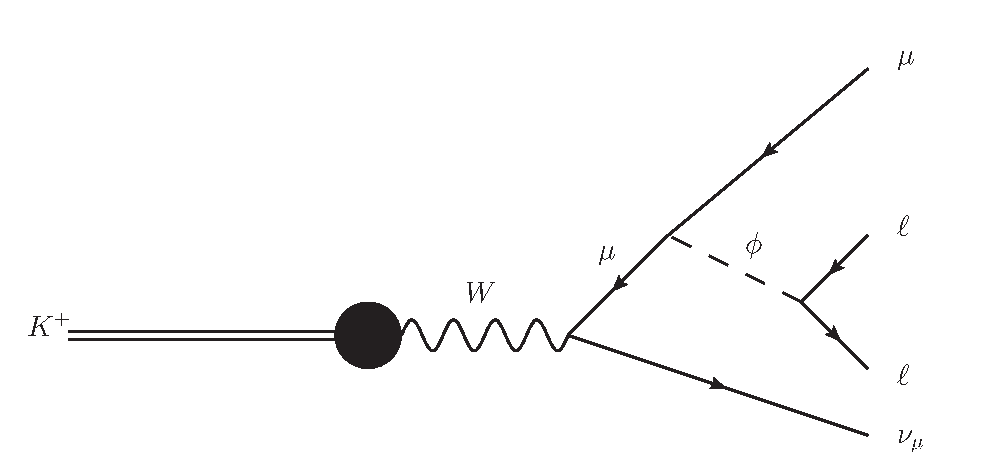
\includegraphics[width=0.6\textwidth]{Figures/feynman_diagrams/k_munull_scalar}
    \caption{Feynman diagram for charged kaon decay through the new scalar. The scalar decays to either an $e^+ e^-$ pair, or a $\mu^+ \mu^-$ pair, depending on the mass available to the scalar, which is taken to be on-shell. The blob represents them form factor for the kaon.}
    \label{fig:kaon_decay_signal}
\end{figure}

We can do this by making use of the Dalitz plot, where one integrates over the squares of the invariant masses of the pairs in the final state.
This means we will integrate over any pair of $m_{\mu\nu}^2$, $m_{\mu\phi}^2$, and $m_{\phi\nu}^2$, instead of over the energies of the outgoing particles.
The reason for doing this is that the matrix element is usually expressed in a simpler fashion using these variables, and the boundaries are easier to define.
It also reads in a more explicitly covariant manner.
The pair of variables we choose to integrate over are $m_{\mu\nu}^2$ and $m_{\mu\phi}^2$.
$m_{\mu\nu}^2$ is chosen because it only appears in the numerator for our process as a simple polynomial when used in conjunction with the other variable.
$m_{\mu\phi}^2$ is chosen because the propagator of the internal muon appears as $\left(m_{\mu\phi}^2 - m_\mu^2\right)^{-1}$, and is naturally expressed in this variable.
In the \emph{Kinematics} section of~\cite{Agashe:2014kda}, the Dalitz plot is specified in these variables as a density of the squared matrix element.
An example plot is shown for $m_\phi = 100\textrm{MeV}$ in Fig.~\ref{fig:dalitz_plot}.

\begin{figure}[h]
    \centering
    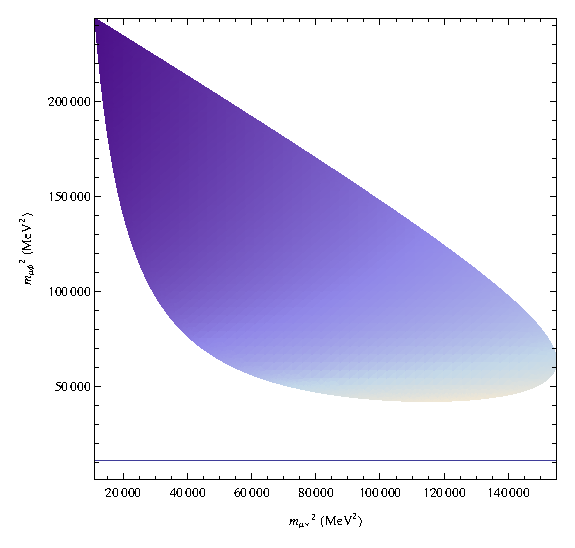
\includegraphics[width=0.5\textwidth]{Figures/kaon/dalitz}
    \caption{Dalitz plot for charged kaon decay. The horizontal line corresponds to the resonant condition $m_{\mu\phi}^2 = m_\mu^2$. As the plot gets lighter, the density gets higher, showing that the density of the amplitude increases as one approaches the resonant condition. Here it is not possible to hit the resonance, but as $m_\phi$ gets very small, we get close to it.}
    \label{fig:dalitz_plot}
\end{figure}

\noindent The allowable region is precisely defined below.

\begin{equation}
\begin{split}
    (m_{\mu\nu}^2)_\textrm{max/min} = m_\mu^2 + \frac{1}{2 m_{\mu\phi}^2} \left(\left(m_K^2 - m_{\mu\phi}^2\right)\left(m_{\mu\phi}^2 - m_\phi^2 + m_\mu^2\right) \pm \right. \\
    \left. \sqrt{\lambda\left(m_{\mu\phi}^2,m_K^2,0\right) \lambda\left(m_{\mu\phi}^2,m_\phi^2,m_\mu^2\right)}\right)
\end{split}
\end{equation}

\noindent $\lambda$ is defined as $\lambda(x,y,z) = x^2 + y^2 + z^2 - 2xy -2xz - 2yz$.
After doing this integration, it is then straightforward to integrate over all allowable values of $m_{\mu\phi}^2 \in [(m_\mu + m_\phi)^2, m_K^2]$, to obtain the total rate.
Carrying out this process yields the width as a function of mass $m_\phi$, and can be seen in Fig.~\ref{fig:kaon_width}.

\begin{figure}[h]
    \centering
    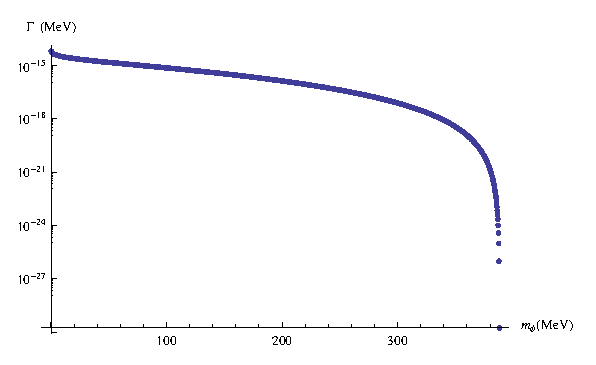
\includegraphics[width=0.5\textwidth]{Figures/kaon/kaon_width}
    \caption{Partial width of $K^+ \rightarrow \mu^+ \mu_\nu \phi$. The coupling was set to $g_{\phi\mu}=1$. There is an increased rate at extremely low energies, and a quick downturn near the kaon less the muon mass, where the phase space closes rapidly.}
    \label{fig:kaon_width}
\end{figure}

Finally, we can use the signal branching ratio combined with our backgrounds to set a limit on the coupling.
The number of signal events we see is given in equation~\ref{eqn:kaon_signal}.

\begin{equation}
    S = N_{K^+}~\textrm{BR}(K^+ \rightarrow \mu^+ \mu_\nu) \frac{\Gamma(K^+ \rightarrow \mu^+ \mu_\nu \phi)}{\Gamma(K^+ \rightarrow \mu^+ \nu_\mu)}
    \label{eqn:kaon_signal}
\end{equation}

\noindent We've chosen to normalize to the two body decay rate here to get rid of any dependence on the kaon form factor.
For the two body decay rate, it is easy to find the following expression

\begin{equation}
    \Gamma(K^+ \rightarrow \mu^+ \nu_\mu) = \frac{1}{8\pi m_K^3}\mathnormal{f}_K^2 \left|V_{us}\right|^2 G_F^2 m_\mu^2 \left(m_K^2 - m_\mu^2\right)^2\textrm{.}
\end{equation}

\noindent In the limit of $m_\phi \ll m_\mu$, we find the following behaviour

\begin{equation}
    \frac{\Gamma(K^+ \rightarrow \mu^+ \nu_\mu \phi)}{\Gamma(K^+ \rightarrow \mu^+ \nu_\mu)} = \frac{1}{4\pi^2} \ln\left(\frac{m_K^2 - m_\mu^2}{2 m_\phi m_\mu} \right)\textrm{.}
\end{equation}

\noindent For $m_\phi = 100\textrm{MeV}$, the branching ratio is $\textrm{BR}(K^+ \rightarrow \mu^+ \nu_\mu \phi) = 1.32\times 10^{-10} \left(g_{\phi\mu}/10^{-4}\right)^2$.

Combining the number of signal events with the number of background events in each background region, we find the limits to follow those in Fig.~\ref{fig:kaon_limits}.
We also assumed an overall signal efficiency of $0.5$.
Since the kaons are boosted, a rough approximation on the maximum angle from the beam any decay products can have is $\theta_\textrm{max} \approx \frac{m_K/2}{p_K} \approx 3\textrm{mrad}$, which stays within the calorimeter's $8.5\textrm{mrad}$ coverage, so most of the decay products producted should pass through the detector.
To be safe though, we choose the efficiency above.
Above the pion mass, the sensitivity drastically decreases.
This is due to the background which we can only poorly estimate in this region until a proper simulation of the background is done, instead of just smearing the events uniformly over the available range.
Right below the pion mass, there is also a downturn visible.
The Dalitz decay quickly vanishes near the kinematic limit, however the other relevant backgrounds in this region are unknown, with the SM process $K^+ \rightarrow \mu^+ \nu_\mu e^+ e^-$ only being measured for $m_{ee} > 150\textrm{MeV}$.
To not mislead the reader here, we simply remove a slice of the parameter space from $130\textrm{MeV}$ up to the pion mass, as there is a relevant background source there, it is just currently unknown how it may affect the sensitivity limits.

\begin{figure}[h]
    \centering
    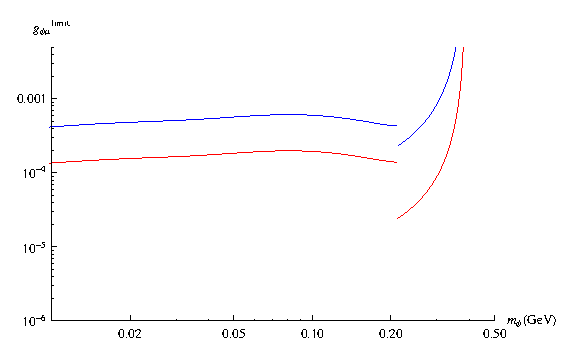
\includegraphics[width=0.6\textwidth]{Figures/limits/kaon_all}
    \caption{Limits on scalar coupling to muon from charged kaon decays. Blue lines correspond to NA48/2 and red to NA62. The three regions each correspond to a different background source, with the Dalitz decay of the $\pi^0$ being dominant below the $\pi^0$ mass, and the irreducible backgrounds to either $\mu^+ \nu_\mu e^+ e^-$ below $2m_\mu$, or $\mu^+ \nu_\mu \mu^+ \mu^-$ above this range to the kinematic limit.}
    \label{fig:kaon_limits}
\end{figure}
